\documentclass[tikz,border=12pt]{standalone}
\usepackage{amsmath}
\usepackage{amssymb}
\usepackage{tikz}
\usetikzlibrary{calc,arrows.meta,decorations.pathmorphing,decorations.pathreplacing,positioning}

\begin{document}
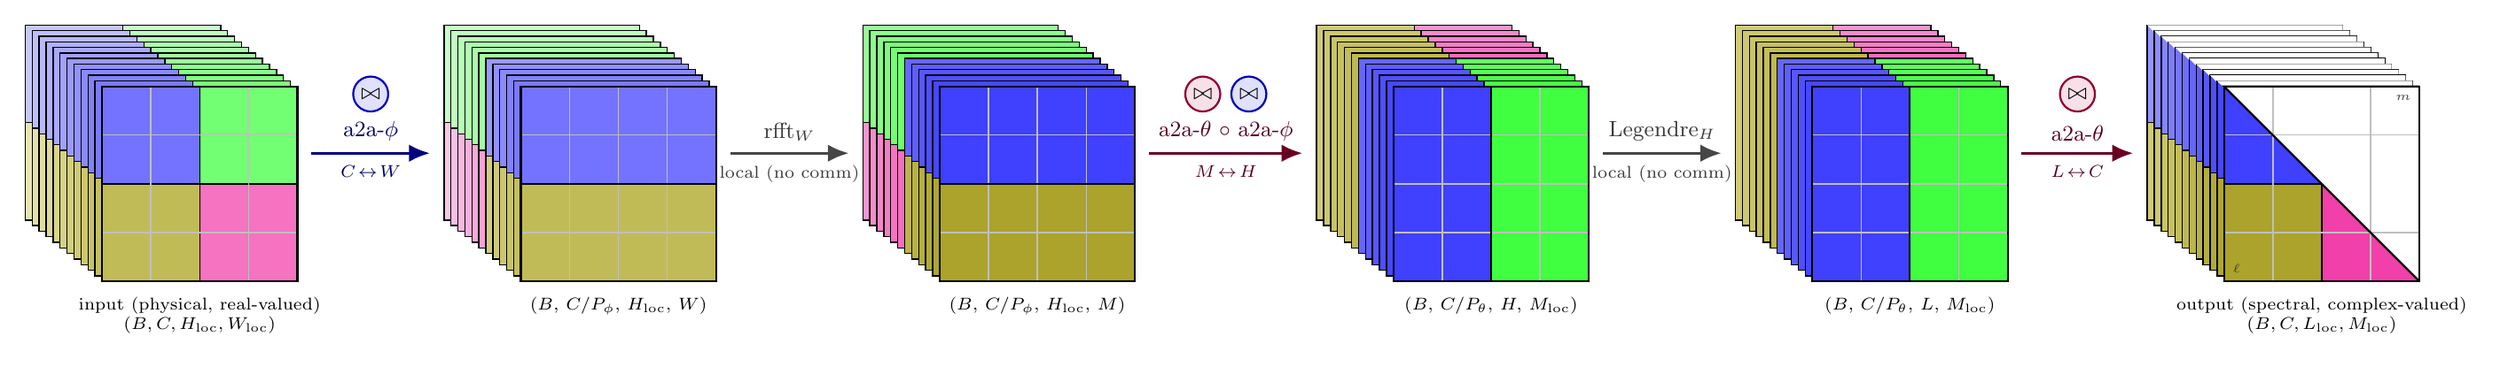
\begin{tikzpicture}[
  font=\sffamily,
  >=Latex,
  line width=0.5pt,
]

% ============================================================================
% Distributed forward SHT — faithful 4 all-to-all version
%
% Code path (DistributedRealSHT.forward in distributed_sht.py):
%   (B, C, H_loc, W_loc)            input — physical, H×W sharded
%     ──[a2a azimuth: C ↔ W]──>     (B, C/P_phi, H_loc, W)
%   rfft over W (local)
%                                   (B, C/P_phi, H_loc, M)
%     ──[a2a azimuth: M ↔ C]──>     (B, C, H_loc, M_loc)
%     ──[a2a polar:   C ↔ H]──>     (B, C/P_theta, H, M_loc)
%   Legendre einsum over H
%                                   (B, C/P_theta, L, M_loc)
%     ──[a2a polar:   L ↔ C]──>     (B, C, L_loc, M_loc)   output — spectral, L×M sharded
%
% 4 all-to-alls total: 2 around the FFT (azimuth), 2 around the Legendre (polar).
% ============================================================================

% ---------- helper: 2x2 yx-sharded grid (4 spatial ranks) ----------
% args: cx, cy, halfwidth, label
\newcommand{\yxgrid}[4]{%
  \fill[blue!25!white,draw=black]    ({#1-#3},{#2})    rectangle ({#1},{#2+#3});
  \fill[green!30!white,draw=black]   ({#1},{#2})       rectangle ({#1+#3},{#2+#3});
  \fill[olive!30!white,draw=black]   ({#1-#3},{#2-#3}) rectangle ({#1},{#2});
  \fill[magenta!25!white,draw=black] ({#1},{#2-#3})    rectangle ({#1+#3},{#2});
  \foreach \i in {-1,1}{
    \draw[gray!50] ({#1+\i*#3/2},{#2-#3}) -- ({#1+\i*#3/2},{#2+#3});
    \draw[gray!50] ({#1-#3},{#2+\i*#3/2}) -- ({#1+#3},{#2+\i*#3/2});
  }
  \draw[thick] ({#1-#3},{#2-#3}) rectangle ({#1+#3},{#2+#3});
  \node[anchor=north,font=\scriptsize,align=center] at (#1,{#2-#3-0.10}) {#4};
}

% ---------- helper: triangular lm-shaped spectral block (L×M sharding) ----------
% Coefficients live in {0 ≤ |m| ≤ ℓ}, so we render the support as a right
% triangle, sub-divided into 4 quadrants using the same NW/NE/SW/SE colours
% so the reader sees how physical ranks map to spectral ranks.
\newcommand{\lmgrid}[4]{%
  \pgfmathsetmacro{\sx}{#1}\pgfmathsetmacro{\sy}{#2}\pgfmathsetmacro{\ss}{#3}
  \fill[blue!18!white,draw=black]    (\sx,         {\sy+\ss/2}) rectangle ({\sx+\ss/2}, {\sy+\ss});
  \fill[green!22!white,draw=black]   ({\sx+\ss/2}, {\sy+\ss/2}) rectangle ({\sx+\ss},   {\sy+\ss});
  \fill[olive!22!white,draw=black]   (\sx,         \sy)         rectangle ({\sx+\ss/2}, {\sy+\ss/2});
  \fill[magenta!18!white,draw=black] ({\sx+\ss/2}, \sy)         rectangle ({\sx+\ss},   {\sy+\ss/2});
  \foreach \i in {1,3}{
    \draw[gray!50] ({\sx+\i*\ss/4},\sy) -- ({\sx+\i*\ss/4},{\sy+\ss});
    \draw[gray!50] (\sx,{\sy+\i*\ss/4}) -- ({\sx+\ss},{\sy+\i*\ss/4});
  }
  \draw[thick] (\sx,\sy) rectangle ({\sx+\ss},{\sy+\ss});
  % mask the upper-triangle (|m| > ℓ) to evoke the spectral support
  \fill[white] ({\sx+\ss},{\sy+\ss}) -- (\sx,{\sy+\ss}) -- ({\sx+\ss},\sy) -- cycle;
  \draw[thick] ({\sx+\ss},{\sy+\ss}) -- (\sx,{\sy+\ss}) -- ({\sx+\ss},\sy);
  \node[font=\tiny,anchor=south west,gray!50!black] at (\sx,\sy) {$\ell$};
  \node[font=\tiny,anchor=north east,gray!50!black] at ({\sx+\ss},{\sy+\ss}) {$m$};
  \node[anchor=north,font=\scriptsize,align=center] at ({\sx+\ss/2},{\sy-0.10}) {#4};
}

% ---------- helper: rank stack-of-stacks (channels split across a comm group) ----------
% Outer offsets = rank axis (4 rank slabs back-to-front); inner offsets = the
% 3 visible "card" cards per rank to suggest the channel/feature stack.
%
% args:
%   #1=anchor x   #2=anchor y   #3=slab width   #4=slab height
%   #5=colour for rank 0   #6=colour for rank 1
%   #7=colour for rank 2   #8=colour for rank 3
\def\dxOut{-0.40}\def\dyOut{0.34}
\def\dxIn{-0.10}\def\dyIn{0.08}
\newcommand{\rankstack}[8]{%
  \foreach \r/\c in {3/#8, 2/#7, 1/#6, 0/#5}{%
    \pgfmathsetmacro{\rxBase}{#1 + \r*\dxOut}%
    \pgfmathsetmacro{\ryBase}{#2 + \r*\dyOut}%
    \foreach \i in {0,1,2}{%
      \pgfmathtruncatemacro{\j}{2-\i}%
      \pgfmathsetmacro{\ox}{\rxBase + \j*\dxIn}%
      \pgfmathsetmacro{\oy}{\ryBase + \j*\dyIn}%
      \pgfmathtruncatemacro{\sh}{55 - \j*12}%
      \fill[\c!\sh!white,draw=black] (\ox,\oy) rectangle ++(#3,#4);%
    }%
  }%
}

% ---------- helper: stacked yxgrid (channels = card stack on a 2x2 spatial grid) ----------
% Same 2x2 spatial sharding as \yxgrid, but stacked N-deep with the
% darker-at-front shading convention used by \rankstack. Use this when
% the channel dimension should be visible alongside the spatial sharding.
%
% args: cx, cy, halfwidth, n-cards, label
\newcommand{\yxstack}[5]{%
  \pgfmathtruncatemacro{\nm}{#4-1}%
  \foreach \k in {0,...,\nm}{%
    \pgfmathtruncatemacro{\j}{\nm-\k}%
    \pgfmathsetmacro{\ox}{#1 + \j*\dxIn}%
    \pgfmathsetmacro{\oy}{#2 + \j*\dyIn}%
    \pgfmathtruncatemacro{\sh}{55 - \j*3}%
    \fill[blue!\sh!white,draw=black]    ({\ox-#3},{\oy})    rectangle ({\ox},{\oy+#3});%
    \fill[green!\sh!white,draw=black]   ({\ox},{\oy})       rectangle ({\ox+#3},{\oy+#3});%
    \fill[olive!\sh!white,draw=black]   ({\ox-#3},{\oy-#3}) rectangle ({\ox},{\oy});%
    \fill[magenta!\sh!white,draw=black] ({\ox},{\oy-#3})    rectangle ({\ox+#3},{\oy});%
  }%
  % subdivisions + thick border on FRONT-most card only
  \foreach \i in {-1,1}{
    \draw[gray!50] ({#1+\i*#3/2},{#2-#3}) -- ({#1+\i*#3/2},{#2+#3});
    \draw[gray!50] ({#1-#3},{#2+\i*#3/2}) -- ({#1+#3},{#2+\i*#3/2});
  }
  \draw[thick] ({#1-#3},{#2-#3}) rectangle ({#1+#3},{#2+#3});
  \node[anchor=north,font=\scriptsize,align=center] at (#1,{#2-#3-0.10}) {#5};
}

% ---------- helper: stacked lmgrid (channels = card stack on the L×M triangle) ----------
% args: lower-left x, lower-left y, side, n-cards, front-saturation, label
\newcommand{\lmstack}[6]{%
  \pgfmathtruncatemacro{\nm}{#4-1}%
  \foreach \k in {0,...,\nm}{%
    \pgfmathtruncatemacro{\j}{\nm-\k}%
    \pgfmathsetmacro{\sx}{#1 + \j*\dxIn}%
    \pgfmathsetmacro{\sy}{#2 + \j*\dyIn}%
    \pgfmathsetmacro{\ss}{#3}%
    \pgfmathtruncatemacro{\sh}{#5 - \j*3}%
    \fill[blue!\sh!white,draw=black]    (\sx,         {\sy+\ss/2}) rectangle ({\sx+\ss/2}, {\sy+\ss});%
    \fill[green!\sh!white,draw=black]   ({\sx+\ss/2}, {\sy+\ss/2}) rectangle ({\sx+\ss},   {\sy+\ss});%
    \fill[olive!\sh!white,draw=black]   (\sx,         \sy)         rectangle ({\sx+\ss/2}, {\sy+\ss/2});%
    \fill[magenta!\sh!white,draw=black] ({\sx+\ss/2}, \sy)         rectangle ({\sx+\ss},   {\sy+\ss/2});%
    % mask the upper-triangle (|m| > ℓ) on every card so they stack as triangles
    \fill[white] ({\sx+\ss},{\sy+\ss}) -- (\sx,{\sy+\ss}) -- ({\sx+\ss},\sy) -- cycle;%
  }%
  % subdivisions + axis ticks + hypotenuse on FRONT-most card only
  \foreach \i in {1,3}{
    \draw[gray!50] ({#1+\i*#3/4},#2) -- ({#1+\i*#3/4},{#2+#3});
    \draw[gray!50] (#1,{#2+\i*#3/4}) -- ({#1+#3},{#2+\i*#3/4});
  }
  \draw[thick] (#1,#2) rectangle ({#1+#3},{#2+#3});
  \draw[thick] ({#1+#3},{#2+#3}) -- (#1,{#2+#3}) -- ({#1+#3},#2);
  \node[font=\tiny,anchor=south west,gray!50!black] at (#1,#2) {$\ell$};
  \node[font=\tiny,anchor=north east,gray!50!black] at ({#1+#3},{#2+#3}) {$m$};
  \node[anchor=north,font=\scriptsize,align=center] at ({#1+#3/2},{#2-0.10}) {#6};
}

% ---------- helper: row-uniform stack (rows colored polar, depth split azimuth) ----
% After the azimuth a2a, W is local per rank — each H row is owned by ONE
% polar rank, but along the channel (= depth) dim the data is split into
% TWO azimuth halves. So:
%   front half of stack  (channels owned by azimuth-0 ranks): blue (top
%       2 rows) over olive (bottom 2 rows)
%   back half of stack   (channels owned by azimuth-1 ranks): green
%       over magenta
% Saturation is the front-card colour intensity; back cards fade as usual.
%
% args: cx, cy, halfwidth, n-cards, front-saturation, label
\newcommand{\rowstack}[6]{%
  \pgfmathtruncatemacro{\nm}{#4-1}%
  \pgfmathtruncatemacro{\half}{#4/2}%
  \foreach \k in {0,...,\nm}{%
    \pgfmathtruncatemacro{\j}{\nm-\k}%
    \pgfmathsetmacro{\ox}{#1 + \j*\dxIn}%
    \pgfmathsetmacro{\oy}{#2 + \j*\dyIn}%
    \pgfmathtruncatemacro{\sh}{#5 - \j*3}%
    \ifnum\j<\half
      % front half: azimuth-0 channels
      \fill[blue!\sh!white,draw=black]    ({\ox-#3},{\oy})    rectangle ({\ox+#3},{\oy+#3});%
      \fill[olive!\sh!white,draw=black]   ({\ox-#3},{\oy-#3}) rectangle ({\ox+#3},{\oy});%
    \else
      % back half: azimuth-1 channels
      \fill[green!\sh!white,draw=black]   ({\ox-#3},{\oy})    rectangle ({\ox+#3},{\oy+#3});%
      \fill[magenta!\sh!white,draw=black] ({\ox-#3},{\oy-#3}) rectangle ({\ox+#3},{\oy});%
    \fi
  }%
  % subdivisions + thick border on FRONT-most card only.
  % NB only the horizontal centerline is a thick "rank divider" — the
  % vertical centerline is gray (since W is local, no rank boundary).
  \foreach \i in {-1,1}{
    \draw[gray!50] ({#1+\i*#3/2},{#2-#3}) -- ({#1+\i*#3/2},{#2+#3});
    \draw[gray!50] ({#1-#3},{#2+\i*#3/2}) -- ({#1+#3},{#2+\i*#3/2});
  }
  \draw[gray!50] (#1,{#2-#3}) -- (#1,{#2+#3});
  \draw[thick] ({#1-#3},#2) -- ({#1+#3},#2);
  \draw[thick] ({#1-#3},{#2-#3}) rectangle ({#1+#3},{#2+#3});
  \node[anchor=north,font=\scriptsize,align=center] at (#1,{#2-#3-0.10}) {#6};
}

% ---------- helper: column-uniform stack (cols colored azimuth, depth split polar)
% After the polar a2a, H is local per rank — each W column is owned by
% ONE azimuth rank, but along the channel (= depth) dim the data is
% split into TWO polar halves.
%   front half  (channels owned by polar-0 ranks): blue (left 2 cols) | green (right 2 cols)
%   back half   (channels owned by polar-1 ranks): olive | magenta
%
% args: cx, cy, halfwidth, n-cards, front-saturation, label
\newcommand{\colstack}[6]{%
  \pgfmathtruncatemacro{\nm}{#4-1}%
  \pgfmathtruncatemacro{\half}{#4/2}%
  \foreach \k in {0,...,\nm}{%
    \pgfmathtruncatemacro{\j}{\nm-\k}%
    \pgfmathsetmacro{\ox}{#1 + \j*\dxIn}%
    \pgfmathsetmacro{\oy}{#2 + \j*\dyIn}%
    \pgfmathtruncatemacro{\sh}{#5 - \j*3}%
    \ifnum\j<\half
      % front half: polar-0 channels
      \fill[blue!\sh!white,draw=black]    ({\ox-#3},{\oy-#3}) rectangle ({\ox},{\oy+#3});%
      \fill[green!\sh!white,draw=black]   ({\ox},{\oy-#3})    rectangle ({\ox+#3},{\oy+#3});%
    \else
      % back half: polar-1 channels
      \fill[olive!\sh!white,draw=black]   ({\ox-#3},{\oy-#3}) rectangle ({\ox},{\oy+#3});%
      \fill[magenta!\sh!white,draw=black] ({\ox},{\oy-#3})    rectangle ({\ox+#3},{\oy+#3});%
    \fi
  }%
  % subdivisions + thick border on FRONT-most card only.
  % NB only the vertical centerline is a thick "rank divider" — the
  % horizontal centerline is gray (since H is local, no rank boundary).
  \foreach \i in {-1,1}{
    \draw[gray!50] ({#1+\i*#3/2},{#2-#3}) -- ({#1+\i*#3/2},{#2+#3});
    \draw[gray!50] ({#1-#3},{#2+\i*#3/2}) -- ({#1+#3},{#2+\i*#3/2});
  }
  \draw[gray!50] ({#1-#3},#2) -- ({#1+#3},#2);
  \draw[thick] (#1,{#2-#3}) -- (#1,{#2+#3});
  \draw[thick] ({#1-#3},{#2-#3}) rectangle ({#1+#3},{#2+#3});
  \node[anchor=north,font=\scriptsize,align=center] at (#1,{#2-#3-0.10}) {#6};
}

% ============================================================================
% LAYOUT — six square blocks (B1-B5 yxgrid-shaped; B6 = lmgrid triangular).
% Same blue/green/olive/magenta rank palette throughout — what changes from
% stage to stage is HOW the colours are laid out on the square, plus a
% saturation drop after each compute step (rfft, Legendre) to mark the
% spectral application of the axis.
% ============================================================================
\def\halfw{1.4}         % all square blocks have halfwidth 1.4 (=> 4x4 effective grid)
% arrow baseline = average of front-card y (=0) and back-card y (=11*dyIn=0.88)
\pgfmathsetmacro{\cY}{(11*\dyIn)/2}

% --------- B1: input (physical, H×W sharded) ---------
% 2x2 rank quadrants — channels are fully replicated across the depth.
\yxstack{0}{0}{\halfw}{12}{input (physical, real-valued)\\$(B,C,H_\text{loc},W_\text{loc})$};

% --------- B2: after a2a #1 — W local, C split on azimuth ---------
% Rows uniform across W (W is now local per rank); the channel dim, now
% split-azimuth, lives in the stack depth (front=azimuth 0, back=azimuth 1).
\def\xB{6.0}
\rowstack{\xB}{0}{\halfw}{12}{55}{$(B,\,C/P_\phi,\,H_\text{loc},\,W)$};

% --------- B3: after rfft over W → modes M ---------
% Same row-uniform sharding as B2 (FFT is local). Saturation BUMPED UP
% from B2 to mark the move into the spectral domain (W → M). All
% downstream blocks carry this same higher saturation — once we're in
% the spectral domain we stay there until the output.
\def\xC{12.0}
\rowstack{\xC}{0}{\halfw}{12}{75}{$(B,\,C/P_\phi,\,H_\text{loc},\,M)$};

% --------- B4: after a2a #2 + a2a #3 — H local, M split azimuth, C split polar ---------
% Columns uniform along H (H is now local); channel dim, now split-polar,
% lives in stack depth (front=polar 0, back=polar 1). Saturation MATCHES
% B3 — a2a doesn't change "how spectral" the data is.
\def\xD{18.5}
\colstack{\xD}{0}{\halfw}{12}{75}{$(B,\,C/P_\theta,\,H,\,M_\text{loc})$};

% --------- B5: after Legendre over H → modes L ---------
% Same column-uniform sharding as B4 (Legendre is local). Saturation
% held at the same level — we're already in the spectral regime.
\def\xE{24.5}
\colstack{\xE}{0}{\halfw}{12}{75}{$(B,\,C/P_\theta,\,L,\,M_\text{loc})$};

% --------- B6: final spectral output (L×M sharded, triangular mask) ---------
% Back to 2x2 rank quadrants — both L and M are now split — plus the
% |m| > ℓ upper-triangle masked to white to evoke the spectral support.
\def\xF{29.0}
\lmstack{\xF}{-1.4}{2.8}{12}{75}{output (spectral, complex-valued)\\$(B,C,L_\text{loc},M_\text{loc})$};

% ============================================================================
% ARROWS + LABELS
% Each B1-B5 block is a 12-card stack at (cx,0) with halfwidth 1.4. Front
% card right edge = cx+1.4; back-most card left edge = cx-1.4+11*dxIn = cx-2.5.
% B6 (lmstack) has lower-left at (xF, -1.4), side 2.8; back-card left = xF-1.1.
% ============================================================================
\def\xPad{0.20}                            % gap between arrow tip and block edge
\pgfmathsetmacro{\xRightOff}{\halfw+\xPad}  %  +1.6 from block centre
\pgfmathsetmacro{\xLeftOff}{\halfw+1.1+\xPad}  %  -2.7 from block centre (back-card)

% --- A1: input → B2 (a2a azimuth) ---
\coordinate (a1s) at ({0+\xRightOff},\cY);
\coordinate (a1e) at ({\xB-\xLeftOff},\cY);
\draw[-{Latex[length=3mm,width=2.5mm]},very thick,blue!50!black] (a1s) -- (a1e);
\node[font=\small,anchor=south,blue!40!black]
  at ($(a1s)!0.5!(a1e)+(0,0.05)$) {a2a-$\phi$};
\node[font=\scriptsize,anchor=north,blue!40!black,align=center]
  at ($(a1s)!0.5!(a1e)+(0,-0.05)$) {$C\!\leftrightarrow\!W$};
\node[draw=blue!75!black,thick,fill=blue!12,circle,inner sep=2pt,font=\small] (i1)
  at ($(a1s)!0.5!(a1e)+(0,0.85)$) {$\bowtie$};

% --- A2: B2 → B3 (rfft, no comm) ---
\coordinate (a2s) at ({\xB+\xRightOff},\cY);
\coordinate (a2e) at ({\xC-\xLeftOff},\cY);
\draw[-{Latex[length=3mm,width=2.5mm]},very thick,gray!55!black] (a2s) -- (a2e);
\node[font=\small,anchor=south,gray!45!black]
  at ($(a2s)!0.5!(a2e)+(0,0.05)$) {rfft$_W$};
\node[font=\scriptsize,anchor=north,gray!45!black,align=center]
  at ($(a2s)!0.5!(a2e)+(0,-0.05)$) {local (no comm)};

% --- A3: B3 → B4 (a2a #2 azimuth, then a2a #3 polar — fused on one arrow) ---
\coordinate (a3s) at ({\xC+\xRightOff},\cY);
\coordinate (a3e) at ({\xD-\xLeftOff},\cY);
\draw[-{Latex[length=3mm,width=2.5mm]},very thick,purple!55!black] (a3s) -- (a3e);
\node[font=\small,anchor=south,purple!45!black]
  at ($(a3s)!0.5!(a3e)+(0,0.05)$) {a2a-${\theta}$ $\circ$ a2a-${\phi}$};
\node[font=\scriptsize,anchor=north,purple!45!black,align=center]
  at ($(a3s)!0.5!(a3e)+(0,-0.05)$) {$M\!\leftrightarrow\!H$};
\node[draw=purple!75!black,thick,fill=purple!12,circle,inner sep=2pt,font=\small] (i2)
  at ($(a3s)!0.35!(a3e)+(0,0.85)$) {$\bowtie$};
\node[draw=blue!75!black,thick,fill=blue!12,circle,inner sep=2pt,font=\small] (i3)
  at ($(a3s)!0.65!(a3e)+(0,0.85)$) {$\bowtie$};

% --- A4: B4 → B5 (Legendre, no comm) ---
\coordinate (a4s) at ({\xD+\xRightOff},\cY);
\coordinate (a4e) at ({\xE-\xLeftOff},\cY);
\draw[-{Latex[length=3mm,width=2.5mm]},very thick,gray!55!black] (a4s) -- (a4e);
\node[font=\small,anchor=south,gray!45!black]
  at ($(a4s)!0.5!(a4e)+(0,0.05)$) {Legendre$_H$};
\node[font=\scriptsize,anchor=north,gray!45!black,align=center]
  at ($(a4s)!0.5!(a4e)+(0,-0.05)$) {local (no comm)};

% --- A5: B5 → B6 (a2a #4 polar) ---
% B6 (lmstack) is lower-left positioned; back-card left edge = xF - 1.1.
\coordinate (a5s) at ({\xE+\xRightOff},\cY);
\coordinate (a5e) at ({\xF-1.1-\xPad},\cY);
\draw[-{Latex[length=3mm,width=2.5mm]},very thick,purple!55!black] (a5s) -- (a5e);
\node[font=\small,anchor=south,purple!45!black]
  at ($(a5s)!0.5!(a5e)+(0,0.05)$) {a2a-${\theta}$};
\node[font=\scriptsize,anchor=north,purple!45!black,align=center]
  at ($(a5s)!0.5!(a5e)+(0,-0.05)$) {$L\!\leftrightarrow\!C$};
\node[draw=purple!75!black,thick,fill=purple!12,circle,inner sep=2pt,font=\small] (i4)
  at ($(a5s)!0.5!(a5e)+(0,0.85)$) {$\bowtie$};

% ============================================================================
% Top annotation: title + comm-count callout
% ============================================================================
%\node[font=\large\bfseries,anchor=south,gray!25!black]
%  at ({\xC}, 3.6)
%  {Distributed forward SHT \,\,(4 all-to-alls)};

%\node[font=\scriptsize,anchor=south,align=center,gray!45!black,text width=11cm]
%  at ({\xC}, 3.0)
%  {\textit{2 a2as bracket the FFT ($\phi$ comm), 2 a2as bracket the Legendre projection ($\theta$ comm).}};

\end{tikzpicture}
\end{document}
